\documentclass{standalone}

\usepackage{tikz}
\usepackage{amsmath,mathtools}

\usepackage{pgfplots}
\usepackage{amsmath,amsthm}
\usepackage{subcaption} 
\usepackage{xspace}
\usepackage{threeparttable}  % For \begin{tablenotes}
\usepackage{multirow}
\usepackage{xcolor}
% Math & symbols


% Units like \SI{10}{m/s}
\usepackage{siunitx}

% Tables
\usepackage{booktabs}

% Figures
\usepackage{graphicx}
\usepackage{subcaption}   % for subfigures

% Floats (for [H] in algorithm)
\usepackage{float}


\usepackage{algorithm}
\usepackage{algpseudocode} % provides algorithmicx/algpseudocode

% Lists (for custom labels S1, S2, …)
\usepackage{enumitem}

\usepackage{multirow}


\usepackage[T1]{fontenc}
\usepackage[tt=false,type1=true]{libertine} % match acmart’s Libertine options
\usepackage[varqu]{zi4}                    % match acmart’s mono setup
\usepackage[libertine]{newtxmath}          % match acmart math (incl. \mathcal)
\def\mathdefault#1{#1}


\AtBeginDocument{%
  \providecommand\BibTeX{{%
    Bib\TeX}}}


\newcommand{\revisionColor}{black}

\usetikzlibrary{intersections, patterns}
\usepgfplotslibrary{groupplots}
\pgfplotsset{compat=1.18}


\usetikzlibrary{positioning}
\usetikzlibrary{ arrows.meta}
\usetikzlibrary{shapes.geometric}
\usetikzlibrary{calc}
\usetikzlibrary{arrows}
\usetikzlibrary{shapes, arrows, positioning, fit, calc, backgrounds, chains,decorations.pathreplacing,hobby}
\usetikzlibrary{mindmap,trees}
\usetikzlibrary{automata,positioning}
\usetikzlibrary{decorations.markings}



\def\distanceXToDT{19}
\def\distanceYToDT{0.4}
\def\distanceL{0.9}
\def\distance2L{2}
\def\innersep{0.4}
\def\squareHeight{0.8}
\def\squareWidth{1.5}
\def\BigSquareWidth{0.45\textwidth}

\tikzset{% UML2 Activity Diagram Styles
  process/.style    = {fill=white,draw, thin, rounded corners=0.8em, minimum height = 12em,
    minimum width = 12em, align=center, inner sep=1em,node distance=4em, yshift=-0.5em},
  object/.style    = {fill=white,draw,thick, rectangle, minimum height = 3em,
    minimum width = 3em, align=center, inner sep=1em,node distance=4em},
  pin/.style    = {fill=white,draw, thin, rectangle, minimum height = 0.6em,
    minimum width = 0.6em, node distance=-1pt, inner sep=0},
  small pin/.style    = {fill=white,draw, thin, rectangle, minimum height = 0.4em,
    minimum width = 0.4em, node distance=-1pt, inner sep=0},
  pin left triangle/.style = {pin,append after command={
      \pgfextra{
        \draw[fill=black] 
          (\tikzlastnode.south east) -- (\tikzlastnode.north east) -- 
          ([xshift=-0.4em]\tikzlastnode.east) -- cycle;
      }
    }
  },
  pin up triangle/.style = {
    pin,
    path picture={
      \draw[fill=white, draw=black, thin]
        ([xshift=-0.3em,yshift=-0.3em]path picture bounding box.center) --
        ([xshift=0.3em,yshift=-0.3em]path picture bounding box.center) --
        ([yshift=0.3em]path picture bounding box.center) -- cycle;
    },
  },
  pin left triangle/.style = {
    pin,
    path picture={
      \draw[fill=black, draw=black]
        ([xshift=0.3em,yshift=-0.3em]path picture bounding box.center) --
        ([xshift=0.3em,yshift=0.3em]path picture bounding box.center) --
        ([xshift=-0.3em]path picture bounding box.center) -- cycle;
    },
  },
  pin right triangle/.style = {
    pin,
    path picture={
      \draw[fill=black, draw=black]
        ([xshift=-0.3em,yshift=-0.3em]path picture bounding box.center) --
        ([xshift=-0.3em,yshift=0.3em]path picture bounding box.center) --
        ([xshift=0.3em]path picture bounding box.center) -- cycle;
    },
  },
}




\begin{document}
      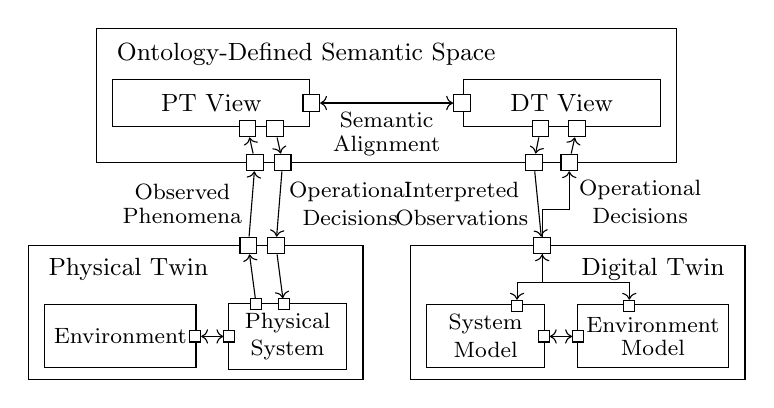
\begin{tikzpicture}[ auto, ]
        
          \node[draw, rectangle, minimum width=\squareWidth cm, minimum height=\squareHeight cm] at (0,0)(E) {\footnotesize Environment};
          
      
          \node[draw, rectangle,   minimum width=\squareWidth cm, minimum height=\squareHeight cm, right= 0.4 cm of E] (PS) {\footnotesize \shortstack{Physical\\ System}};


        \node [small pin,right=of E,yshift=-0.0cm, xshift=
        -0.06cm](ETablR){};

        %\node [small pin,above=of E,yshift=-0.06cm, xshift=0.3cm](ETablA){};


        \node [small pin,left=of PS,yshift=-0.0cm, xshift=
        0.06cm](PSTablL){};
        
        \node [small pin,above=of PS,yshift=-0.06cm, xshift= -0.4cm](PSTablA){};

        \node [small pin,above=of PS,yshift=-0.06cm, xshift= -0.05cm](PSTablA2){};

        \node [rectangle, draw=black, fit={(PS) (E)}, minimum width=3cm, inner sep=0.2 cm,yshift = 0.3 cm, minimum height=1.7cm,  label={[anchor=north west, xshift=4pt, yshift=-1pt]north west:\small Physical Twin}](PT){}; 


        \node [pin,above=of PT,yshift=-0.08cm, xshift=
        0.67cm](PTab){};

        \node [pin,above=of PT,yshift=-0.08cm, xshift=
        1.02cm](PTab2){};

        \draw[<->] (ETablR) -- (PSTablL);

        \draw[->] (PSTablA) -- (PTab);
        \draw[<-] (PSTablA2) -- (PTab2);

        %\draw (ETablA) -- ++(0,0.3) -| (PTab);


        

         \node[draw, rectangle, minimum width=\squareWidth cm, minimum height=\squareHeight cm, right = 1 cm of PS](SM) {\footnotesize \shortstack{System \\ Model}};
         \node[draw, rectangle,   minimum width=\squareWidth cm, minimum height=\squareHeight cm, right= 0.4 cm of SM] (EM) {\footnotesize \shortstack{Environment \\ Model}};

        \node [small pin,right=of SM,yshift=-0.0cm, xshift=
        -0.06cm](SMTablR){};

        \node [small pin,above=of SM,yshift=-0.06cm, xshift=
        0.4cm](SMTablA){};


        \node [small pin,left=of EM,yshift=-0.0cm, xshift=
        0.06cm](EMTablL){};
        
        \node [small pin,above=of EM,yshift=-0.06cm, xshift= -0.3cm](EMTablA){};

        \node [rectangle, draw=black, fit={(SM) (EM)}, minimum width=3cm, inner sep=0.2 cm,yshift = 0.3 cm, minimum height=1.7cm,  label={[anchor=north east, xshift=-4pt, yshift=-1pt]north east:\small Digital Twin}](DT){}; 


        \node [pin,above=of DT,yshift=-0.08cm, xshift=
        -0.45cm](DTab){};
        


      
        
      
        \draw[<->] (SMTablR) -- (EMTablL);
      
        \draw[<->] (SMTablA) --++(0,0.3)-| (DTab);
      
        \draw[<-] (EMTablA) -- ++(0,0.3) -| (DTab);


        \node[rectangle, draw, minimum width=2.5cm, inner sep=0.2,minimum height=0.6cm, above= 1.5 cm of PT, xshift = 0.2cm] (PTView) {\small PT View};

        \node [pin,below=of PTView,yshift=0.06cm, xshift= 0.46cm](PTViewTabB){};
        \node [pin,below=of PTView,yshift=0.06cm, xshift= 0.81cm](PTViewTabB2){};
         \node [pin,right=of PTView,yshift=0.00cm, xshift= -0.065cm](PTViewTabR){};

        \node[rectangle, draw, minimum width=2.5cm, inner sep=0.2,minimum height=0.6cm, above= 1.5 cm of DT, xshift = -0.2cm] (DTView) {\small DT View};
         \node [pin,below=of DTView,yshift=0.06cm, xshift= 0.19cm](DTViewTabB){};
         \node [pin,below=of DTView,yshift=0.06cm, xshift= -0.27cm](DTViewTabB2){};

         \node [pin,left=of DTView,yshift=0.00cm, xshift= 0.065cm](DTViewTabL){};



        \node [rectangle, draw=black, fit={(PTView) (DTView)}, minimum width=3cm, inner sep=0.2 cm,yshift = 0.1 cm, minimum height=1.7cm,  label={[anchor=north west, xshift=4pt, yshift=-2pt]north west:\small Ontology-Defined Semantic Space}](OSS){}; 

        \node[pin, below=of OSS,yshift=0.08cm, xshift=-1.67cm](OSSTabPT){};

        \node[pin, below=of OSS,yshift=0.08cm, xshift=-1.32cm](OSSTabPT2){};


        \node[pin, below=of OSS,yshift=0.08cm, xshift=2.32cm](OSSTabDT){};

        \node[pin, below=of OSS,yshift=0.08cm, xshift=1.87cm](OSSTabDT2){};


        

        \draw[<-] (OSSTabPT) -- node[left]{\footnotesize \shortstack{Observed \\Phenomena}}(PTab);

        \draw[->] (OSSTabPT2) -- node[right]{\footnotesize \shortstack{Operational\\Decisions}}(PTab2);


          \draw[<-] (OSSTabDT) |-node[right, yshift = 0.1cm]{\footnotesize \shortstack{Operational \\ Decisions}} ++(0,-0.6) -| (DTab);

          \draw[->] (OSSTabDT2) -- node[left]{\footnotesize \shortstack{Interpreted \\ Observations}}(DTab);


          \draw[<-] (PTViewTabB) -- (OSSTabPT);
          \draw[->] (PTViewTabB2) -- (OSSTabPT2);
          \draw[<-] (DTViewTabB) -- (OSSTabDT);
          \draw[->] (DTViewTabB2) -- (OSSTabDT2);

          \draw[<->] (PTViewTabR) -- node[below] {\footnotesize \shortstack{Semantic \\Alignment}}  (DTViewTabL) ;
        
        
\end{tikzpicture}
\end{document}